\chapter{Architettura del software}

\section{Architettura logica}

\dfn{Architettura}{
    La progettazione OO è  basata su diversi strati architetturali,
    come uno strato UI, uno strato di logica applicativa (o "del dominio") e così via.
}

\nt{L'architettura può essere mostrata sotto forma di diagrammi UML.}

\ex{Package UML}{
    \begin{center}
        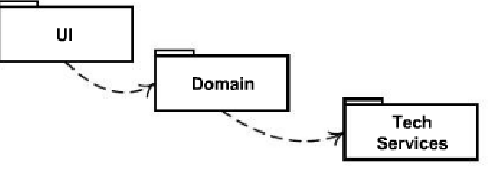
\includegraphics[scale=0.5]{images/PackageUML.png}
    \end{center}
}

\dfn{Architettura logica}{
    L'\newfancyglitter{architettura logica} di un sistema
    software è la macro-organizzazione su larga scala delle 
    classi in package (o namespace), sottoinsiemi e strati.
}

\nt{Non vengono prese decisioni su come gli elementi sono distribuiti
sui processi o sui vari computer fisici di una rete (\fancyglitter{platform independent architecture}).}

\cor{Layer (o Strato)}{
    Un layer è un gruppo di classi software, packages, sottosistemi con responsabilità
    condivisa su un aspetto importante del sistema.
}

\subsubsection{Gli strati comprendono:}

\begin{itemize}
    \item [$\Rightarrow$] \fancyglitter{UI (User Interface)}: strato che si occupa dell'interazione con l'utente;
    \item [$\Rightarrow$] \fancyglitter{Application logic} (o "domain object"): oggetti software che rappresentano concetti di dominio;
    \item [$\Rightarrow$] \fancyglitter{Technical services}: oggetti e sottosistemi che forniscono servizi tecnici (es. persistenza, sicurezza, ecc.);
\end{itemize}

\subsubsection{Rappresentazioni di strati:}
    \begin{figure}[!h]
        \centering
        \subfloat[Packeges UML]{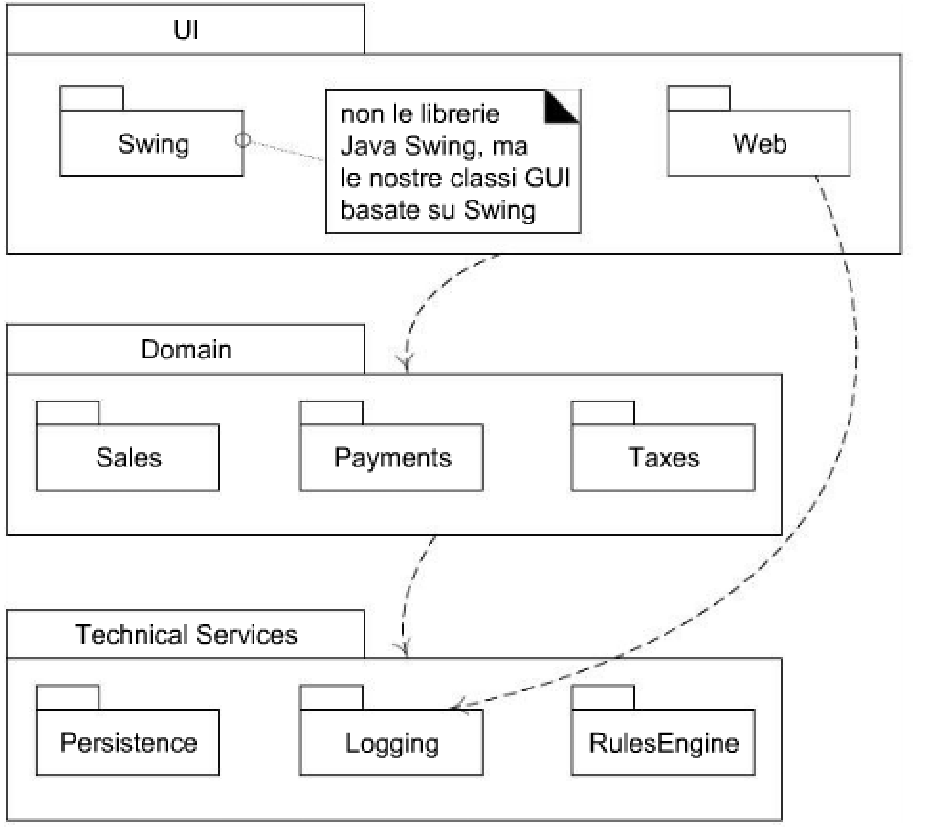
\includegraphics[scale = 0.25]{images/UMLPackage.png}} 
        \subfloat[Relativo codice]{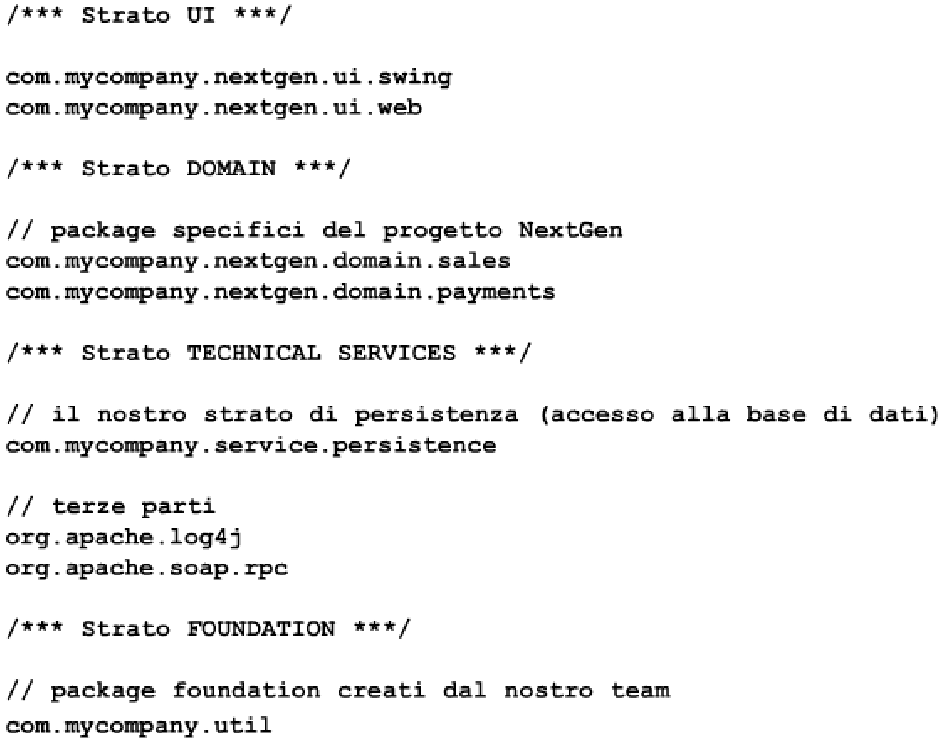
\includegraphics[scale = 0.25]{images/PackageCode.png}}
    \end{figure}

\dfn{Architettura a strati}{
    L'obiettivo di un'\newfancyglitter{architettura a strati} è la suddivisione di un sistema complesso
    in un insieme di elementi software che possano essere sviluppati e modificati in modo indipendente.
}

\cor{Separation of concerns}{
    La separazione degli interessi:

    \begin{itemize}
        \item [$\Rightarrow$] Riduce l'accoppiamento e le dipendenze;
        \item [$\Rightarrow$] Aumenta la possibilità di riuso;
        \item [$\Rightarrow$] Facilita la manutenzione e l'evoluzione del sistema;
        \item [$\Rightarrow$] Aumenta la chiarezza.
    \end{itemize}
}

\cor{Alta coesione}{
    In uno strato le responsabilità degli oggetti devono essere fortemente
    collegate tra loro, ma non essere mischiate con quelle di altri strati.
}

\nt{Questi due principi verranno ripresi in GRASP, vedi capitolo \ref{GRASP}.}

\pagebreak

\ex{Architettura a strati}{
    \begin{center}
        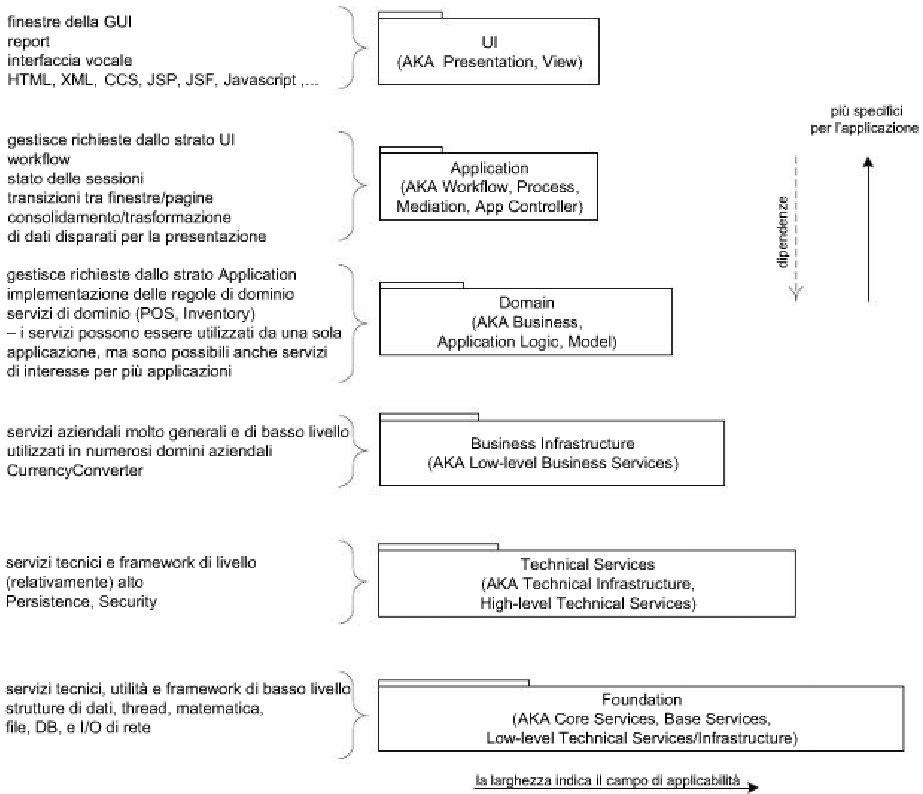
\includegraphics[scale=0.45]{images/Architettura a strati.png}
    \end{center}

}


\section{Strato del dominio}

\qs{}{Come va progettata la logica applicativa con gli oggetti?}

\paragraph{Risposta:} Si creano oggetti software con nomi e informazioni simili
al Dominio del mondo reale e assegnare a essi le responsabilità della logica applicativa.

\dfn{Oggetto del Dominio}{
    Un \newfancyglitter{oggetto del dominio} è un oggetto software che rappresenta un concetto del dominio del problema.

    Ha una logica applicativa o di business correlata.
}

\nt{Ispirandosi al Modello del Dominio si ha un basso salto rappresentazionale che
rende più facile e veloce l'implementazione.}

\ex{Strato di Dominio e Modello di Dominio}{

    \begin{center}
        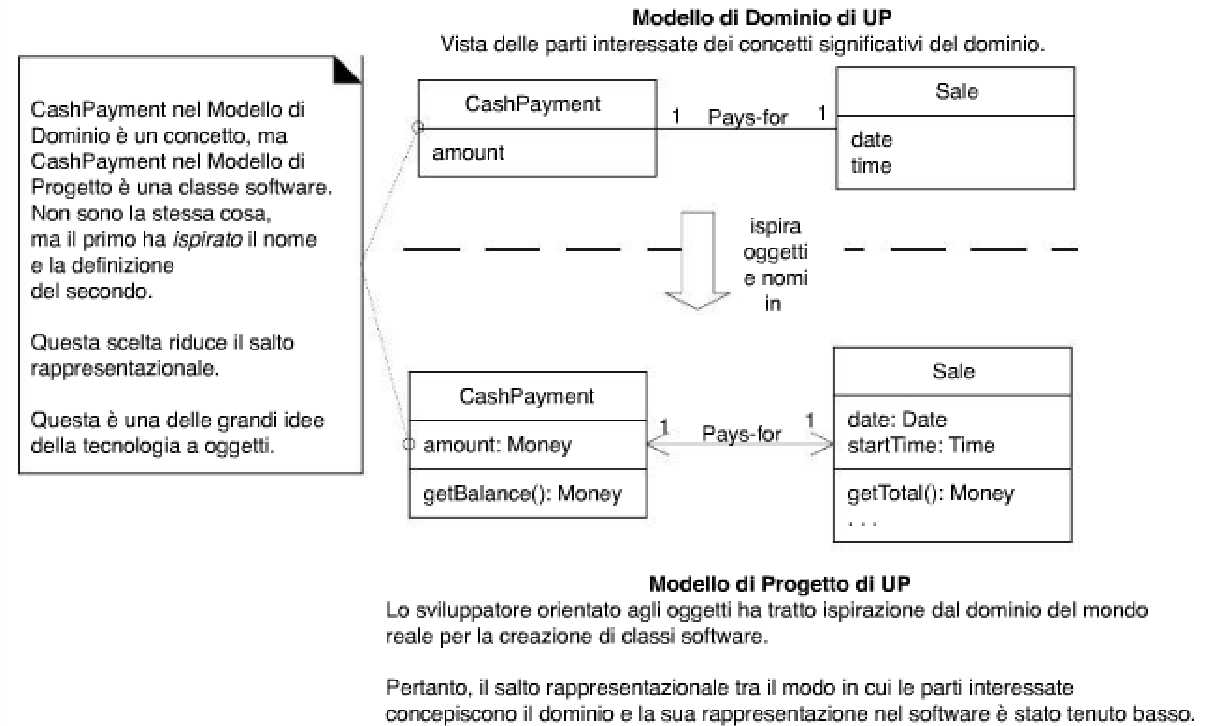
\includegraphics[scale=0.35]{images/Modello.png}
    \end{center}
}

\ex{Strati e Partizioni}{
    \begin{center}
        \includegraphics[scale=0.35]{images/Strati e Partizioni.png}
    \end{center}
}

\section{Separazione Modello-Vista}

\dfn{Principio di separazione Modello-Vista}{
    \begin{itemize}
        \item [\textcolor{red}{\XSolidBrush}] Non relazionare o accoppiare oggetti non UI con oggetti UI.
        \item [\textcolor{red}{\XSolidBrush}] Non incapsulare la logica applicativa in metodi UI.
        \item [\textcolor{green}{\Checkmark}] Le finestre appartengono a una specifica applicazione, mentre
        gli oggetti non UI possono venire riutilizzati in nuove applicazioni o associati a nuove interfacce.
        \item [\textcolor{green}{\Checkmark}] Gli oggetti UI inizializzano elementi UI, ricevono eventi UI e
        delegano le richieste della logica dell'applicazione agli oggetti non UI.
    \end{itemize}
}

\nt{
    \begin{itemize}
        \item [$\Rightarrow$] Il Modello è lo strato degli oggetti del dominio;
        \item [$\Rightarrow$] La Vista è lo strato UI.
    \end{itemize}

    Questo principio è alla base del pattern MVC\footnote{Visto nel corso "Programmazione III".}.
}

\subsubsection{Ulteriori considerazioni:}

\begin{itemize}
    \item [$\Rightarrow$] Le classi di dominio incapsulano le informazioni e il comportamento della logica applicativa;
    \item [$\Rightarrow$] Le classi della vista sono leggere, sono responsabili dell'inpute e dell'output, ma non mantengono dati.
\end{itemize}

\subsubsection{Vantaggi:}

\begin{itemize}
    \item [$\Rightarrow$] Favorire la definizione coesa dei modelli;
    \item [$\Rightarrow$] Consentire lo sviluppo separaro;
    \item [$\Rightarrow$] Minimizzare l'impatto sullo strato del dominio;
    \item [$\Rightarrow$] Consentire di connettere facilmente nuove viste;
    \item [$\Rightarrow$] Consentire l'esecuzione dello strato di modello indipendentemente dallo strato UI;
    \item [$\Rightarrow$] Consentire un \textit{porting} facile dello strato di modello a un altro framework UI.
\end{itemize}

\ex{SSD e UI}{
    \begin{center}
        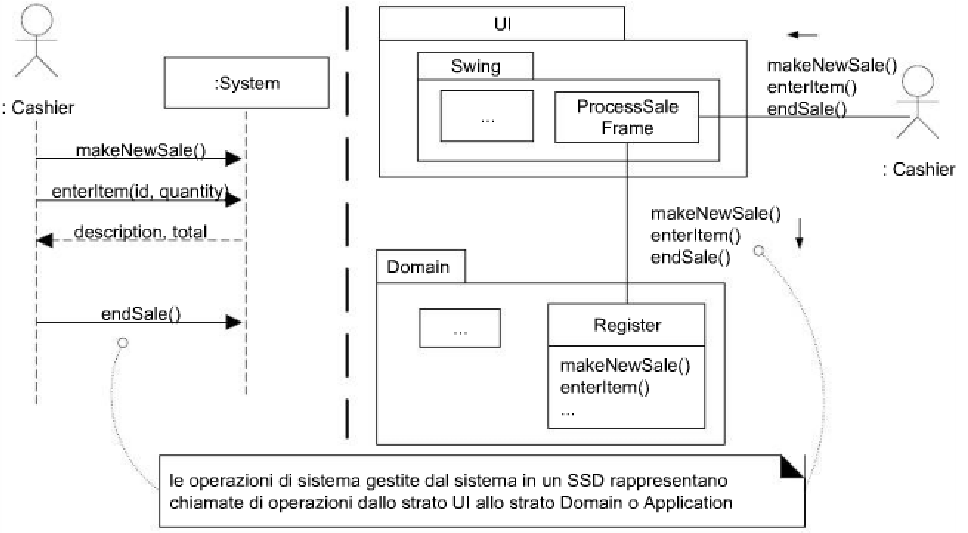
\includegraphics[scale=0.3]{images/SSD e UI.png}
    \end{center}
}
